%% This style is provided for the ICSE 2015 main conference,
%% ICSE 2015 co-located events, and ICSE 2015 workshops.

%% bare_conf_ICSE15.tex
%% V1.4
%% 2014/05/22


%% This is a skeleton file demonstrating the use of IEEEtran.cls
%% (requires IEEEtran.cls version 1.7 or later) with an IEEE conference paper.
%%
%% Support sites:
%% http://www.michaelshell.org/tex/ieeetran/
%% http://www.ctan.org/tex-archive/macros/latex/contrib/IEEEtran/
%% and
%% http://www.ieee.org/

%%*************************************************************************
%% Legal Notice:
%% This code is offered as-is without any warranty either expressed or
%% implied; without even the implied warranty of MERCHANTABILITY or
%% FITNESS FOR A PARTICULAR PURPOSE!
%% User assumes all risk.
%% In no event shall IEEE or any contributor to this code be liable for
%% any damages or losses, including, but not limited to, incidental,
%% consequential, or any other damages, resulting from the use or misuse
%% of any information contained here.
%%
%% All comments are the opinions of their respective authors and are not
%% necessarily endorsed by the IEEE.
%%
%% This work is distributed under the LaTeX Project Public License (LPPL)
%% ( http://www.latex-project.org/ ) version 1.3, and may be freely used,
%% distributed and modified. A copy of the LPPL, version 1.3, is included
%% in the base LaTeX documentation of all distributions of LaTeX released
%% 2003/12/01 or later.
%% Retain all contribution notices and credits.
%% ** Modified files should be clearly indicated as such, including  **
%% ** renaming them and changing author support contact information. **
%%
%% File list of work: IEEEtran.cls, IEEEtran_HOWTO.pdf, bare_adv.tex,
%%                    bare_conf.tex, bare_jrnl.tex, bare_jrnl_compsoc.tex
%%*************************************************************************

% *** Authors should verify (and, if needed, correct) their LaTeX system  ***
% *** with the testflow diagnostic prior to trusting their LaTeX platform ***
% *** with production work. IEEE's font choices can trigger bugs that do  ***
% *** not appear when using other class files.                            ***
% The testflow support page is at:
% http://www.michaelshell.org/tex/testflow/



% Note that the a4paper option is mainly intended so that authors in
% countries using A4 can easily print to A4 and see how their papers will
% look in print - the typesetting of the document will not typically be
% affected with changes in paper size (but the bottom and side margins will).
% Use the testflow package mentioned above to verify correct handling of
% both paper sizes by the user's LaTeX system.
%
% Also note that the "draftcls" or "draftclsnofoot", not "draft", option
% should be used if it is desired that the figures are to be displayed in
% draft mode.
%
\documentclass[conference]{IEEEtran}
%
% If IEEEtran.cls has not been installed into the LaTeX system files,
% manually specify the path to it like:
% \documentclass[conference]{../sty/IEEEtran}



\usepackage{tabularx}


% Some very useful LaTeX packages include:
% (uncomment the ones you want to load)


% *** MISC UTILITY PACKAGES ***
%
%\usepackage{ifpdf}
% Heiko Oberdiek's ifpdf.sty is very useful if you need conditional
% compilation based on whether the output is pdf or dvi.
% usage:
% \ifpdf
%   % pdf code
% \else
%   % dvi code
% \fi
% The latest version of ifpdf.sty can be obtained from:
% http://www.ctan.org/tex-archive/macros/latex/contrib/oberdiek/
% Also, note that IEEEtran.cls V1.7 and later provides a builtin
% \ifCLASSINFOpdf conditional that works the same way.
% When switching from latex to pdflatex and vice-versa, the compiler may
% have to be run twice to clear warning/error messages.






% *** CITATION PACKAGES ***
%
%\usepackage{cite}
% cite.sty was written by Donald Arseneau
% V1.6 and later of IEEEtran pre-defines the format of the cite.sty package
% \cite{} output to follow that of IEEE. Loading the cite package will
% result in citation numbers being automatically sorted and properly
% "compressed/ranged". e.g., [1], [9], [2], [7], [5], [6] without using
% cite.sty will become [1], [2], [5]--[7], [9] using cite.sty. cite.sty's
% \cite will automatically add leading space, if needed. Use cite.sty's
% noadjust option (cite.sty V3.8 and later) if you want to turn this off.
% cite.sty is already installed on most LaTeX systems. Be sure and use
% version 4.0 (2003-05-27) and later if using hyperref.sty. cite.sty does
% not currently provide for hyperlinked citations.
% The latest version can be obtained at:
% http://www.ctan.org/tex-archive/macros/latex/contrib/cite/
% The documentation is contained in the cite.sty file itself.






% *** GRAPHICS RELATED PACKAGES ***
%
\ifCLASSINFOpdf
  \usepackage[pdftex]{graphicx}
  % declare the path(s) where your graphic files are
  \graphicspath{{images/}}
  % and their extensions so you won't have to specify these with
  % every instance of \includegraphics
  % \DeclareGraphicsExtensions{.pdf,.jpeg,.png}
\else
  % or other class option (dvipsone, dvipdf, if not using dvips). graphicx
  % will default to the driver specified in the system graphics.cfg if no
  % driver is specified.
  % \usepackage[dvips]{graphicx}
  % declare the path(s) where your graphic files are
  % \graphicspath{{../eps/}}
  % and their extensions so you won't have to specify these with
  % every instance of \includegraphics
  % \DeclareGraphicsExtensions{.eps}
\fi
% graphicx was written by David Carlisle and Sebastian Rahtz. It is
% required if you want graphics, photos, etc. graphicx.sty is already
% installed on most LaTeX systems. The latest version and documentation can
% be obtained at:
% http://www.ctan.org/tex-archive/macros/latex/required/graphics/
% Another good source of documentation is "Using Imported Graphics in
% LaTeX2e" by Keith Reckdahl which can be found as epslatex.ps or
% epslatex.pdf at: http://www.ctan.org/tex-archive/info/
%
% latex, and pdflatex in dvi mode, support graphics in encapsulated
% postscript (.eps) format. pdflatex in pdf mode supports graphics
% in .pdf, .jpeg, .png and .mps (metapost) formats. Users should ensure
% that all non-photo figures use a vector format (.eps, .pdf, .mps) and
% not a bitmapped formats (.jpeg, .png). IEEE frowns on bitmapped formats
% which can result in "jaggedy"/blurry rendering of lines and letters as
% well as large increases in file sizes.
%
% You can find documentation about the pdfTeX application at:
% http://www.tug.org/applications/pdftex





% *** MATH PACKAGES ***
%
%\usepackage[cmex10]{amsmath}
% A popular package from the American Mathematical Society that provides
% many useful and powerful commands for dealing with mathematics. If using
% it, be sure to load this package with the cmex10 option to ensure that
% only type 1 fonts will utilized at all point sizes. Without this option,
% it is possible that some math symbols, particularly those within
% footnotes, will be rendered in bitmap form which will result in a
% document that can not be IEEE Xplore compliant!
%
% Also, note that the amsmath package sets \interdisplaylinepenalty to 10000
% thus preventing page breaks from occurring within multiline equations. Use:
%\interdisplaylinepenalty=2500
% after loading amsmath to restore such page breaks as IEEEtran.cls normally
% does. amsmath.sty is already installed on most LaTeX systems. The latest
% version and documentation can be obtained at:
% http://www.ctan.org/tex-archive/macros/latex/required/amslatex/math/





% *** SPECIALIZED LIST PACKAGES ***
%
%\usepackage{algorithmic}
% algorithmic.sty was written by Peter Williams and Rogerio Brito.
% This package provides an algorithmic environment fo describing algorithms.
% You can use the algorithmic environment in-text or within a figure
% environment to provide for a floating algorithm. Do NOT use the algorithm
% floating environment provided by algorithm.sty (by the same authors) or
% algorithm2e.sty (by Christophe Fiorio) as IEEE does not use dedicated
% algorithm float types and packages that provide these will not provide
% correct IEEE style captions. The latest version and documentation of
% algorithmic.sty can be obtained at:
% http://www.ctan.org/tex-archive/macros/latex/contrib/algorithms/
% There is also a support site at:
% http://algorithms.berlios.de/index.html
% Also of interest may be the (relatively newer and more customizable)
% algorithmicx.sty package by Szasz Janos:
% http://www.ctan.org/tex-archive/macros/latex/contrib/algorithmicx/




% *** ALIGNMENT PACKAGES ***
%
%\usepackage{array}
% Frank Mittelbach's and David Carlisle's array.sty patches and improves
% the standard LaTeX2e array and tabular environments to provide better
% appearance and additional user controls. As the default LaTeX2e table
% generation code is lacking to the point of almost being broken with
% respect to the quality of the end results, all users are strongly
% advised to use an enhanced (at the very least that provided by array.sty)
% set of table tools. array.sty is already installed on most systems. The
% latest version and documentation can be obtained at:
% http://www.ctan.org/tex-archive/macros/latex/required/tools/


%\usepackage{mdwmath}
%\usepackage{mdwtab}
% Also highly recommended is Mark Wooding's extremely powerful MDW tools,
% especially mdwmath.sty and mdwtab.sty which are used to format equations
% and tables, respectively. The MDWtools set is already installed on most
% LaTeX systems. The lastest version and documentation is available at:
% http://www.ctan.org/tex-archive/macros/latex/contrib/mdwtools/


% IEEEtran contains the IEEEeqnarray family of commands that can be used to
% generate multiline equations as well as matrices, tables, etc., of high
% quality.


%\usepackage{eqparbox}
% Also of notable interest is Scott Pakin's eqparbox package for creating
% (automatically sized) equal width boxes - aka "natural width parboxes".
% Available at:
% http://www.ctan.org/tex-archive/macros/latex/contrib/eqparbox/





% *** SUBFIGURE PACKAGES ***
%\usepackage[tight,footnotesize]{subfigure}
% subfigure.sty was written by Steven Douglas Cochran. This package makes it
% easy to put subfigures in your figures. e.g., "Figure 1a and 1b". For IEEE
% work, it is a good idea to load it with the tight package option to reduce
% the amount of white space around the subfigures. subfigure.sty is already
% installed on most LaTeX systems. The latest version and documentation can
% be obtained at:
% http://www.ctan.org/tex-archive/obsolete/macros/latex/contrib/subfigure/
% subfigure.sty has been superceeded by subfig.sty.



%\usepackage[caption=false]{caption}
%\usepackage[font=footnotesize]{subfig}
% subfig.sty, also written by Steven Douglas Cochran, is the modern
% replacement for subfigure.sty. However, subfig.sty requires and
% automatically loads Axel Sommerfeldt's caption.sty which will override
% IEEEtran.cls handling of captions and this will result in nonIEEE style
% figure/table captions. To prevent this problem, be sure and preload
% caption.sty with its "caption=false" package option. This is will preserve
% IEEEtran.cls handing of captions. Version 1.3 (2005/06/28) and later
% (recommended due to many improvements over 1.2) of subfig.sty supports
% the caption=false option directly:
%\usepackage[caption=false,font=footnotesize]{subfig}
%
% The latest version and documentation can be obtained at:
% http://www.ctan.org/tex-archive/macros/latex/contrib/subfig/
% The latest version and documentation of caption.sty can be obtained at:
% http://www.ctan.org/tex-archive/macros/latex/contrib/caption/




% *** FLOAT PACKAGES ***
%
%\usepackage{fixltx2e}
% fixltx2e, the successor to the earlier fix2col.sty, was written by
% Frank Mittelbach and David Carlisle. This package corrects a few problems
% in the LaTeX2e kernel, the most notable of which is that in current
% LaTeX2e releases, the ordering of single and double column floats is not
% guaranteed to be preserved. Thus, an unpatched LaTeX2e can allow a
% single column figure to be placed prior to an earlier double column
% figure. The latest version and documentation can be found at:
% http://www.ctan.org/tex-archive/macros/latex/base/



%\usepackage{stfloats}
% stfloats.sty was written by Sigitas Tolusis. This package gives LaTeX2e
% the ability to do double column floats at the bottom of the page as well
% as the top. (e.g., "\begin{figure*}[!b]" is not normally possible in
% LaTeX2e). It also provides a command:
%\fnbelowfloat
% to enable the placement of footnotes below bottom floats (the standard
% LaTeX2e kernel puts them above bottom floats). This is an invasive package
% which rewrites many portions of the LaTeX2e float routines. It may not work
% with other packages that modify the LaTeX2e float routines. The latest
% version and documentation can be obtained at:
% http://www.ctan.org/tex-archive/macros/latex/contrib/sttools/
% Documentation is contained in the stfloats.sty comments as well as in the
% presfull.pdf file. Do not use the stfloats baselinefloat ability as IEEE
% does not allow \baselineskip to stretch. Authors submitting work to the
% IEEE should note that IEEE rarely uses double column equations and
% that authors should try to avoid such use. Do not be tempted to use the
% cuted.sty or midfloat.sty packages (also by Sigitas Tolusis) as IEEE does
% not format its papers in such ways.





% *** PDF, URL AND HYPERLINK PACKAGES ***
%
\usepackage{url}
% url.sty was written by Donald Arseneau. It provides better support for
% handling and breaking URLs. url.sty is already installed on most LaTeX
% systems. The latest version can be obtained at:
% http://www.ctan.org/tex-archive/macros/latex/contrib/misc/
% Read the url.sty source comments for usage information. Basically,
% \url{my_url_here}.





% *** Do not adjust lengths that control margins, column widths, etc. ***
% *** Do not use packages that alter fonts (such as pslatex).         ***
% There should be no need to do such things with IEEEtran.cls V1.6 and later.
% (Unless specifically asked to do so by the journal or conference you plan
% to submit to, of course. )

%\usepackage{verbatim}

\usepackage{listings}

% correct bad hyphenation here
\hyphenation{op-tical net-works semi-conduc-tor}

\newcommand{\smu}{\emph{sun.misc.Unsafe}}


\begin{document}
%
% paper title
% can use linebreaks \\ within to get better formatting as desired
\title{Mining Ultra-Large-Scale Software Repositories and StackOverflow database to study \emph{sun.misc.Unsafe} API usage patterns in Java applications}


% author names and affiliations
% use a multiple column layout for up to three different
% affiliations
%\author{\IEEEauthorblockN{Michael Shell}
%\IEEEauthorblockA{School of Electrical and\\Computer Engineering\\
%Georgia Institute of Technology\\
%Atlanta, Georgia 30332--0250\\
%Email: http://www.michaelshell.org/contact.html}
%\and
%\IEEEauthorblockN{Homer Simpson}
%\IEEEauthorblockA{Twentieth Century Fox\\
%Springfield, USA\\
%Email: homer@thesimpsons.com}
%\and
%\IEEEauthorblockN{James Kirk\\ and Montgomery Scott}
%\IEEEauthorblockA{Starfleet Academy\\
%San Francisco, California 96678-2391\\
%Telephone: (800) 555--1212\\
%Fax: (888) 555--1212}}

% conference papers do not typically use \thanks and this command
% is locked out in conference mode. If really needed, such as for
% the acknowledgment of grants, issue a \IEEEoverridecommandlockouts
% after \documentclass

% for over three affiliations, or if they all won't fit within the width
% of the page, use this alternative format:
%
\author{\IEEEauthorblockN{Luis Mastrangelo\IEEEauthorrefmark{1},
Matthias Hauswirth\IEEEauthorrefmark{1} and
Nate Nystrom\IEEEauthorrefmark{1}}
\IEEEauthorblockA{\IEEEauthorrefmark{1}Faculty of Informatics, University of Lugano}
}




% use for special paper notices
%\IEEEspecialpapernotice{(Invited Paper)}




% make the title area
\maketitle


\begin{abstract}
%\boldmath

The Java language and Java Virtual Machine (JVM) evolved over time to satisfy the needs for millons of developers worldwide.
Performance is one of the main drivers why the Java language changed.
One of this changes is the addition of an undocumented class, \smu{}, provided by Oracle.
Although \smu{} allows the developer to access low-level programming features, its use is extremely dangerous.
In some cases, its use can lead to a crash of the JVM.

In this paper, we study how effectively this API is used in industry.
To carry out our study, we mine ultra-large-scale software repositories and the StackOverflow database.
The goal of our study is to answer the following question: Why and how the Unsafe API is used in Java projects?

Our aim is to devise safer alternatives to \smu{} on the JVM to improve programmer productivity.

\end{abstract}
% IEEEtran.cls defaults to using nonbold math in the Abstract.
% This preserves the distinction between vectors and scalars. However,
% if the conference you are submitting to favors bold math in the abstract,
% then you can use LaTeX's standard command \boldmath at the very start
% of the abstract to achieve this. Many IEEE journals/conferences frown on
% math in the abstract anyway.

% no keywords




% For peer review papers, you can put extra information on the cover
% page as needed:
% \ifCLASSOPTIONpeerreview
% \begin{center} \bfseries EDICS Category: 3-BBND \end{center}
% \fi
%
% For peerreview papers, this IEEEtran command inserts a page break and
% creates the second title. It will be ignored for other modes.
\IEEEpeerreviewmaketitle




\section{Introduction} \label{sec:introduction}

Performance is the main reason for Unsafe.

Trend using unsafe methods. But what for? Certainly you can do everithing without Unsafe API, so why using it? The key is performance.

We searched for Boa \cite{Dyer-Nguyen-Rajan-Nguyen-13}


GHTorrent \cite{Gousi13} provide GitHub quering but for metadata, not source code mining, true?


\subsection{Subsection Heading Here}
Subsection text here.


\subsubsection{Subsubsection Heading Here}

%\verbatiminput{../boa-client/unsafe.boa}


This demo file is intended to serve as a ``starter file''
for IEEE conference papers produced under \LaTeX\ using
IEEEtran.cls version 1.7 and later.
% You must have at least 2 lines in the paragraph with the drop letter
% (should never be an issue)
I wish you the best of success.

\hfill mds

\hfill January 11, 2007


\section{Related Work} \label{sec:relatedwork}

GHTorrent \cite{Gousi13} provide GitHub quering but for metadata, not source code mining, true?

Lean GHtorrent \cite{GousiosMSR2014b} provides mining of GitHub repositories, but for a limit impose by GitHub, only 1,000 repositories can be queried.

Boa
For source code mining we searched in Boa \cite{Dyer-Nguyen-Rajan-Nguyen-13}. 


\cite{Dyer-Rajan-Nguyen-Nguyen-14}

Paul Sandoz estimates how Unsafe is used~\cite{psandoz14}, but only provides a survey.

Several research work uses \smu{} in their implementation.

As far as we know, no prior work shows how the \smu{} is used in industry.


\section{Mining Boa infrastructure} \label{sec:methodologyboa}

In this section we describe our methodology to mine the data we used for our analysis.
We first begin describing how we mined source code repositories. The next section describes how we analysed the Stackoverflow database.

The complete scripts and results used for our study are available online~\footnote{\url{https://bitbucket.org/acuarica/java-unsafe-analysis}}.

\subsection{Static usage}

For source code mining we searched in Boa \cite{Dyer-Nguyen-Rajan-Nguyen-13}. 
The BOA infrastructure allows the user to navigate the parsed AST of source code.
Notice that BOA does not provide type resolution analysis.
Therefore we develop some heuristics to determine where and how \smu{} is used.

The following assumptions hold:
\begin{itemize}
\item \smu{} class is \texttt{final} 
\item inherits directly from \texttt{java.lang.Object}
\item Its public methods (except for \texttt{getUnsafe}) are instance methods
\end{itemize}

Thus, our Boa script~\footnote{\url{https://bitbucket.org/acuarica/java-unsafe-analysis/raw/master/unsafe-analysis/unsafe.boa}} looks for \texttt{sun.misc.Unsafe} as either an import or fully qualified name where a type may appear.
In case that we found a use of \smu{} we proceed to determine which method is used.
If \smu{} is found in a compilation unit, then all call sites in the compilation unit are analysed.
If a call site target is one of the \smu{} methods, then we can conclude that \smu{} is used and that method is called.

\subsection{Reflection usage}

What happens if \smu{} is used through reflection?
Sometimes this API is used through reflection to avoid the compilation dependency (remember that \smu{} is not part of the public API).

For instance, listing~\ref{lst:reflection} shows how to take the address size of the host machine.
First it obtains an instance of \smu{} by reflection.
Then, again by reflection, invoke the method \texttt{addressSize}, which returns the address size of the host machine.


%\definecolor{codegreen}{rgb}{0,0.6,0}
%\definecolor{codegray}{rgb}{0.5,0.5,0.5}
%\definecolor{codepurple}{rgb}{0.58,0,0.82}
%\definecolor{backcolour}{rgb}{0.95,0.95,0.92}
 
\lstdefinestyle{java}{
    language=Java,
 %   backgroundcolor=\color{backcolour},   
%    commentstyle=\color{codegreen},
%    keywordstyle=\color{magenta},
  %  numberstyle=\tiny\color{codegray},
%    stringstyle=\color{codepurple},
    basicstyle=\footnotesize,
    breakatwhitespace=false,         
    breaklines=true,                 
    captionpos=b,                    
    keepspaces=true,                 
%    numbers=left,                    
%    numbersep=5pt,                  
    showspaces=false,                
    showstringspaces=false,
    showtabs=false,                  
    tabsize=2,
    frame=shadowbox
}

\lstset{style=java}
\lstset{escapechar=§}

\begin{lstlisting}[caption=Use of sun.misc.Unsafe with reflection,label=lst:reflection]
Class<?> cls = Class.forName("sun.misc.Unsafe");
Field theUnsafe = cls.getDeclaredField("theUnsafe");
theUnsafe.setAccessible(true);
Object unsafe = theUnsafe.get(null);
Method method = cls.getMethod("addressSize");
Object value = method.invoke(unsafe);
int addressSize = ((Number) value).intValue();
\end{lstlisting}

We are aware of this situation and also look for the string literal \texttt{"sun.misc.Unsafe"} to see when it is used through reflection.

\subsection{Avoiding duplicates}

Usually a code repository has branches, to allow the team to introduce new features without interrupt the main source of development.
In Boa, all \smu{} uses are reported, regardless if it is the same file in different branches.
Sometimes it happens that the same file, with the same uses, has different package in different branches.

Therefore we need to take into account this situation.
To determine if a file is a duplicate in another branch, we look for the same file name and uses, if we found the same file and the same uses, we assume that the file is in a branch and we exclude it.

\subsection{JDK forks}

Our script also retrieves the package of the compilation unit.
With the package we can determine if the compilation unit belongs to a JDK implementation.

\subsection{Metadata}

Also we are interested in some metadata information.
For each project that uses \smu{}, either statically or dinamically, our Boa script also retrieves :
\begin{itemize}
\item the size of the project (in number of AST nodes)
\item the number of revisions in the repository.
\item the lifetime of the repository (time from the first to the last commit)
\end{itemize}

It is possible to group methods in \smu{} by functionality.
Table \ref{table:groups} shows all methods (without overloads) grouped by functionality.


\begin{table}[ht]
\centering
\caption{Functional groups of \smu{}}
\label{table:groups}
\begin{tabular}{|r|l|l|} \hline
Group  & Methods \\ \hline \hline
Array  & arrayBaseOffset arrayIndexScale \\ \hline
CAS    & compareAndSwapInt compareAndSwapLong \\
       & compareAndSwapObject \\ \hline
Class  & defineAnonymousClass defineClass ensureClassInitialized \\ \hline
Get    & getBoolean getByte getChar getDouble getFloat getInt \\
       & getIntVolatile getLoadAverage getLong getLongVolatile \\
       & getObject getObjectVolatile getShort getBooleanVolatile \\
       & getDoubleVolatile getFloatVolatile getByteVolatile \\
       & getCharVolatile getShortVolatile \\ \hline
Memory & addressSize allocateMemory copyMemory freeMemory \\
       & getAddress pageSize putAddress \\ 
       & reallocateMemory setMemory \\ \hline
Offset & fieldOffset objectFieldOffset staticFieldBase staticFieldOffset \\ \hline
Park   & park unpark \\ \hline
Put    & putBoolean putByte putChar putDouble putFloat putInt \\
       & putIntVolatile putLong putLongVolatile putObject \\
       & putObjectVolatile putOrderedInt putOrderedLong \\
       & putOrderedObject putShort putCharVolatile \\ 
       & putOrderedInt putBooleanVolatile putShortVolatile \\ 
       & putFloatVolatile putByteVolatile putDoubleVolatile \\ \hline
Single & allocateInstance throwException \\ \hline
Monitor & monitorEnter monitorExit tryMonitorEnter \\ \hline

\end{tabular}
\end{table}

% Not used methods
% monitorEnter monitorExit tryMonitorEnter
% defineAnonymousClass
% shouldBeInitialized ???

% getBooleanVolatile getDoubleVolatile getFloatVolatile getByteVolatile getCharVolatile getShortVolatile

% putOrderedInt putBooleanVolatile putShortVolatile putFloatVolatile putByteVolatile putDoubleVolatile putCharVolatile



\section{Mining StackOverflow} \label{sec:methodologyso}

In this section we describe our methodology to retrieve the data we used for our analysis.
We first begin describing how we mined source code repositories and then how we analysed the Stackoverflow database.

The complete scripts and results used for our study are available online~\footnote{\url{https://bitbucket.org/acuarica/java-unsafe-analysis}}.

\subsection{Source Code repositories}

For source code mining we searched in Boa \cite{Dyer-Nguyen-Rajan-Nguyen-13}. 
The BOA infrastructure allows the user to navigate the parsed AST of source code.

Our Boa script looks for \texttt{sun.misc.Unsafe} as either an import or fully qualified name where a type may appear.
In case that we found a use of \smu{} we proceed to determine which method is used.


It is possible to group methods in \smu{} by functionality.
Table \ref{table:groups} shows all methods (without overloads) grouped by functionality.


\begin{table}[ht]
\centering
\caption{Functional groups of \smu{}}
\label{table:groups}
\begin{tabular}{|r|l|l|} \hline
Group  & Methods \\ \hline \hline
Array  & arrayBaseOffset arrayIndexScale \\ \hline
CAS    & compareAndSwapInt compareAndSwapLong \\
       & compareAndSwapObject \\ \hline
Class  & defineAnonymousClass defineClass ensureClassInitialized \\ \hline
Get    & getBoolean getByte getChar getDouble getFloat getInt \\
       & getIntVolatile getLoadAverage getLong getLongVolatile \\
       & getObject getObjectVolatile getShort getBooleanVolatile \\
       & getDoubleVolatile getFloatVolatile getByteVolatile \\
       & getCharVolatile getShortVolatile \\ \hline
Memory & addressSize allocateMemory copyMemory freeMemory \\
       & getAddress pageSize putAddress \\ 
       & reallocateMemory setMemory \\ \hline
Offset & fieldOffset objectFieldOffset staticFieldBase staticFieldOffset \\ \hline
Park   & park unpark \\ \hline
Put    & putBoolean putByte putChar putDouble putFloat putInt \\
       & putIntVolatile putLong putLongVolatile putObject \\
       & putObjectVolatile putOrderedInt putOrderedLong \\
       & putOrderedObject putShort putCharVolatile \\ 
       & putOrderedInt putBooleanVolatile putShortVolatile \\ 
       & putFloatVolatile putByteVolatile putDoubleVolatile \\ \hline
Single & allocateInstance throwException \\ \hline
Monitor & monitorEnter monitorExit tryMonitorEnter \\ \hline

\end{tabular}
\end{table}

% Not used methods
% monitorEnter monitorExit tryMonitorEnter
% defineAnonymousClass
% shouldBeInitialized ???

% getBooleanVolatile getDoubleVolatile getFloatVolatile getByteVolatile getCharVolatile getShortVolatile

% putOrderedInt putBooleanVolatile putShortVolatile putFloatVolatile putByteVolatile putDoubleVolatile putCharVolatile


\subsubsection*{Reflection}

%\begin{verbatim}
%Class<?> unsafeClass = Class.forName("sun.misc.Unsafe");
%Field unsafeField = unsafeClass.getDeclaredField("theUnsafe");
%unsafeField.setAccessible(true);
%Object unsafe = unsafeField.get(null);
%int addressSize = ((Number) %unsafeClass.getMethod("addressSize").invoke(unsafe)).intValue();
%\end{verbatim}

What happens with other uses such as reflection? It is not detected but it uses Unsafe. There should be a way to measure this kind of use.

Look for problematic uses of the API, and some use patterns.


\subsection{Stackoverflow}

Google search for sun.misc.unsafe site:stackoverflow.com
returns about 1,360 results.


\section{Results} \label{sec:results}

The Figure~\ref{fig:java-over-total} shows the pie.

\begin{figure}[htb]
\centering
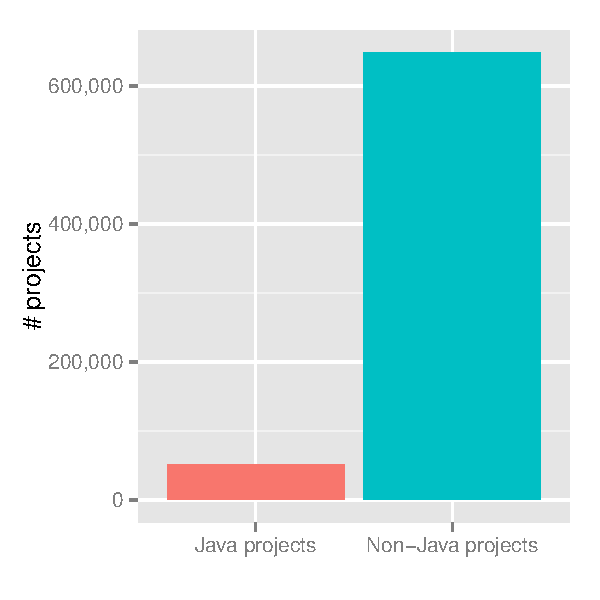
\includegraphics[width=\columnwidth]{unsafe-plot-java-over-total}
\caption{\# Java and non-Java projects} \label{fig:java-over-total}
\end{figure}

\begin{figure}[htb]
\centering
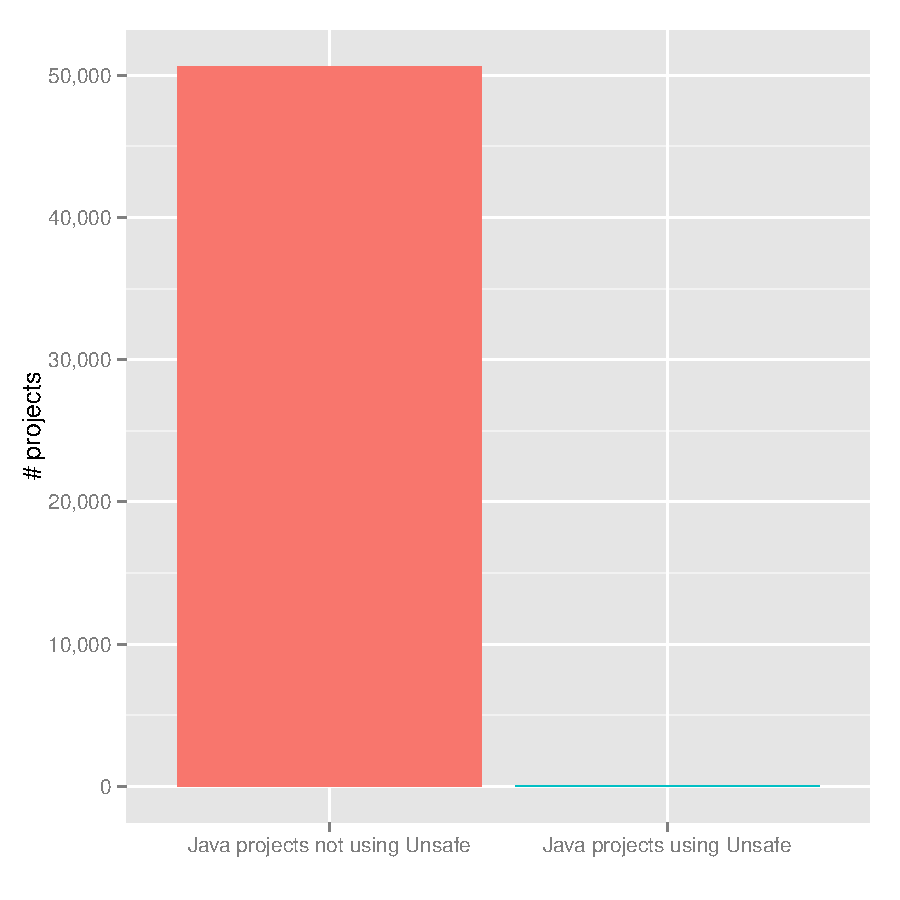
\includegraphics[width=\columnwidth]{unsafe-plot-unsafe-over-java}
\caption{Project using unsafe} \label{fig:unsafe-over-java}
\end{figure}

The figure~\ref{fig:usage} shows how many times a method is called. Grouped by functional group.

\begin{figure*}[htb]
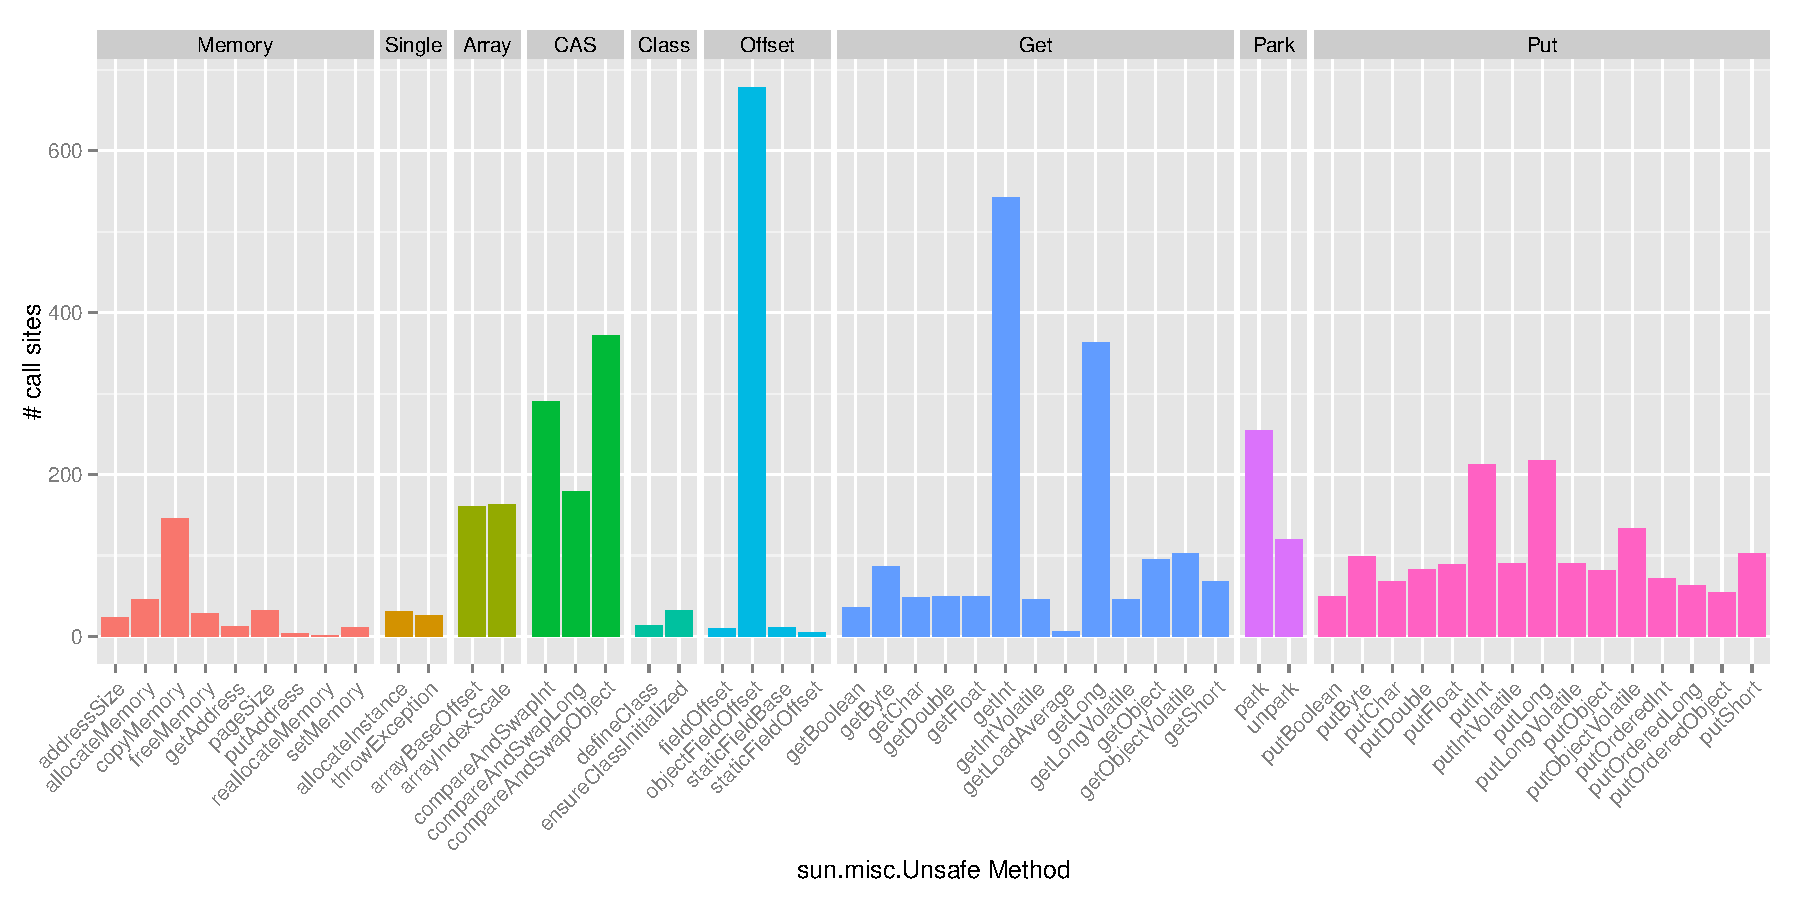
\includegraphics[width=\textwidth]{unsafe-plot-usage}
\caption{sun.misc.Unsafe methods usage} \label{fig:usage}
\end{figure*}

The most called is \texttt{objectFieldOffset}. Because the result is then used by many other calls to Unsafe.


\begin{table*}[htb]
\centering
\caption{Java projects using \smu{}}  \label{table:projects}
\begin{tabularx}{\textwidth}{|r|l|X|r|r|r|r|r|} \hline    

 \# & Name & Description & \# Revisions & \# AST Nodes & Lifetime & \# smU Calls & \# smU Literal \\ \hline
  1 & adtools & Amiga Development Tools (adtools) & 466 & 14911 k & 6 years  & 421 & \\ 
  2 & amino & Concurrent Building Block & 691 & 255 k & 4 years  &  53 & \\ 
  3 & amock & Java Mock libarary for static method &   3 & 13 k &  21 days &  14 & \\ 
  4 & android & Android on PXA270   & 146 & 4836 k &  7 months  &  77 & \\ 
  5 & aojunit & An aspect-oriented extension to JUnit   &   5 & 1 k & 1 day &   1 & \\ 
  6 & archaiosjava & Scalable and fast libraries for Java  &  17 & 11 k &  14 days & 102 & \\ 
  7 & beanlib & Java Bean Library  & 854 & 119 k & 6 years  &   4 & \\ 
  8 & caloriecount & Track what you eat  & 202 & 352 k &  5 months &  10 & \\ 
  9 & cegcc & CeGCC - Cross development for Pocket PC  & 1449 & 2203 k & 4 years & 101 & \\ 
  10 & cgnu & CGNU (Clean GNU)  &  60 & 2135 k &  1 month & 101 & \\ 
  11 & classreach & Identifies unused Java classes and methods  &  69 & 196 k & 2 years & 10 & \\ 
  12 & clipc & Library for IPC  & 278 & 228 k &  6 months &  10 & \\ 
  13 & concutest & Tools to test concurrent Java programs & 14 & 550 k & 2 years  & 185 & \\ 
  14 & ec & ec-gin Europe China Grid InterNetworking    &   9 & 635 k &  2 month  &  10 & 1 \\ 
  15 & essence & Essence Java Framework    & 293 & 157 k & 2 years &  75 & \\ 
  16 & essentialbudget & Essential Budget   &  55 & 60 k &  4 months &  20 & 2 \\ 
  17 & glassbox & Troubleshooting and monitoring agent  & 458 & 99 k & 4 years &   1 & \\ 
  18 & grinder & Load testing framework  & 4334 & 770 k & 11 years  &   6 & \\ 
  19 & high & Highly Scalable Java   &  78 & 37 k & 2 years &  37 & \\ 
  20 & hlv & Collection of high level view plugins for eclipse & 278 & 33 k & 7 months & & 4 \\   
  21 & ikvm & JVM for .NET Framework and Mono   & 3980 & 531 k & 10 years & 123 & \\ 
  22 & jadoth & abstraction utils and frameworks   & 2922 & 619 k & 3 years & 949 & \\ 
  23 & janetdev & Ja.NET - Java Development Tools for .NET   & 366 & 10034 k &  2 years & 280 & \\ 
  24 & janux & Java directly on the Linux Kernel  &  25 & 564 k & 1 month  &  10 & \\ 
  25 & java & Lightweight Java Game Library  & 3841 & 571 k & 11 years  &   6 & \\ 
  26 & javapathfinder & Verifies Java bytecode programs & 4038 & 9952 k & 6 years & & 4 \\ 
  27 & javapayload & Payloads to be used for post-exploitation  &  92 & 74 k & 2 years & 28 & 1 \\ 
  28 & jaxlib & Platform independent Java library  & 3208 & 5405 k & 11 years & 42 & 3 \\ 
  29 & jigcell & Computational biology problem solving & 5286 & 3573 k & 8 years & & 3 \\ 
  30 & jikesrvm & The Jikes Research Virtual Machine (RVM) & 16068 & 9026 k & 10 years & 32 & 16\\ 
  31 & jnode & JNode: new Java Operating System  & 11972 & 44401 k & 10 years  & 2104 & \\ 
  32 & jon & Java Object Notation  & 118 & 29 k &  8 months &  3 & \\ 
  33 & jprovocateur & RAD for Ajax applications in Java & 934 & 197 k &  2 year &  10 & 2 \\ 
  34 & junitrecorder & Record test cases  &  18 & 34 k &  3 months  &   1 & \\ 
  35 & katta & Lucene in the cloud  & 478 & 169 k &  1 year &  31 & \\ 
  36 & l2next & L2 Private Server code   &  22 & 39 k &  1 month &  26 & \\ 
  37 & lockss & Lots of Copies Keep Stuff Safe & 23048 & 11551 k & 11 years & & 2 \\ 
  38 & neurogrid & P2P Bookmark Organiser  & 738 & 337 k & 5 years &   2 & \\ 
  39 & osfree & osFree operating system   & 1124 & 119 k & 5 years &  96 & \\ 
  40 & ps2toolchain & Toolchain for the Playstation 2's   &   8 & 4298 k &  1 day & 202 & \\ 
  41 & simulaeco & Semester project  &  66 & 136 k &  4 months  &  10 & 2 \\ 
  42 & snarej & Snare's Not A Risc OS Emulator in Java  &  82 & 111 k &  27 days &  19 & \\ 
  43 & statewalker & Graph traversing library   & 432 & 477 k & 3 years &  36 & 2 \\ 
  44 & takatuka & TakaTuka Java Virtual Machine   & 2637 & 1176 k & 3 years & 107 & \\ 
  45 & timelord & A tool for estimating and tracking time   & 546 & 697 k &  2 year &  40 & \\ 
  46 & ucl & A final year project by UCL students &  70 & 1639 k &  3 months & & 1 \\ 
  47 & vcb & Component Based Development tool   & 2446 & 602 k & 3 years &  11 & \\ 
  48 & x10 & Experimental language for DARPA/HPCS   & 25432 & 12292 k & 9 years & 279 & \\ 
  49 & xbeedriver & Driver for the ZigBee network  &   6 & 119 k &  3 days &  10 & 2\\ 
  \hline
\end{tabularx}
\end{table*}




\section{Conclusions} \label{sec:conclusions}

Although the current use of \smu{} seems low in SourceForge, it is important to notice the snapshot is from September 2013.
It would be interesting to apply the same analysis but to the current GitHub source code database.
Unfortunately at the moment we could not find any full dataset from GuitHub.

We strongly believe that this study will help us to develop our language.
% use section* for acknowledgement

\section*{Acknowledgments}

The first author was supported by Swiss National Science Foundation grant CRSII2\_136225.



% no \IEEEPARstart


% An example of a floating figure using the graphicx package.
% Note that \label must occur AFTER (or within) \caption.
% For figures, \caption should occur after the \includegraphics.
% Note that IEEEtran v1.7 and later has special internal code that
% is designed to preserve the operation of \label within \caption
% even when the captionsoff option is in effect. However, because
% of issues like this, it may be the safest practice to put all your
% \label just after \caption rather than within \caption{}.
%
% Reminder: the "draftcls" or "draftclsnofoot", not "draft", class
% option should be used if it is desired that the figures are to be
% displayed while in draft mode.
%
%\begin{figure}[!t]
%\centering
%\includegraphics[width=2.5in]{myfigure}
% where an .eps filename suffix will be assumed under latex,
% and a .pdf suffix will be assumed for pdflatex; or what has been declared
% via \DeclareGraphicsExtensions.
%\caption{Simulation Results}
%\label{fig_sim}
%\end{figure}

% Note that IEEE typically puts floats only at the top, even when this
% results in a large percentage of a column being occupied by floats.


% An example of a double column floating figure using two subfigures.
% (The subfig.sty package must be loaded for this to work.)
% The subfigure \label commands are set within each subfloat command, the
% \label for the overall figure must come after \caption.
% \hfil must be used as a separator to get equal spacing.
% The subfigure.sty package works much the same way, except \subfigure is
% used instead of \subfloat.
%
%\begin{figure*}[!t]
%\centerline{\subfloat[Case I]\includegraphics[width=2.5in]{subfigcase1}%
%\label{fig_first_case}}
%\hfil
%\subfloat[Case II]{\includegraphics[width=2.5in]{subfigcase2}%
%\label{fig_second_case}}}
%\caption{Simulation results}
%\label{fig_sim}
%\end{figure*}
%
% Note that often IEEE papers with subfigures do not employ subfigure
% captions (using the optional argument to \subfloat), but instead will
% reference/describe all of them (a), (b), etc., within the main caption.


% An example of a floating table. Note that, for IEEE style tables, the
% \caption command should come BEFORE the table. Table text will default to
% \footnotesize as IEEE normally uses this smaller font for tables.
% The \label must come after \caption as always.
%
%\begin{table}[!t]
%% increase table row spacing, adjust to taste
%\renewcommand{\arraystretch}{1.3}
% if using array.sty, it might be a good idea to tweak the value of
% \extrarowheight as needed to properly center the text within the cells
%\caption{An Example of a Table}
%\label{table_example}
%\centering
%% Some packages, such as MDW tools, offer better commands for making tables
%% than the plain LaTeX2e tabular which is used here.
%\begin{tabular}{|c||c|}
%\hline
%One & Two\\
%\hline
%Three & Four\\
%\hline
%\end{tabular}
%\end{table}


% Note that IEEE does not put floats in the very first column - or typically
% anywhere on the first page for that matter. Also, in-text middle ("here")
% positioning is not used. Most IEEE journals/conferences use top floats
% exclusively. Note that, LaTeX2e, unlike IEEE journals/conferences, places
% footnotes above bottom floats. This can be corrected via the \fnbelowfloat
% command of the stfloats package.






% trigger a \newpage just before the given reference
% number - used to balance the columns on the last page
% adjust value as needed - may need to be readjusted if
% the document is modified later
%\IEEEtriggeratref{8}
% The "triggered" command can be changed if desired:
%\IEEEtriggercmd{\enlargethispage{-5in}}

% references section

% can use a bibliography generated by BibTeX as a .bbl file
% BibTeX documentation can be easily obtained at:
% http://www.ctan.org/tex-archive/biblio/bibtex/contrib/doc/
% The IEEEtran BibTeX style support page is at:
% http://www.michaelshell.org/tex/ieeetran/bibtex/
\bibliographystyle{IEEEtran}
% argument is your BibTeX string definitions and bibliography database(s)
%\bibliography{IEEEabrv,../bib/paper}
%
% <OR> manually copy in the resultant .bbl file
% set second argument of \begin to the number of references
% (used to reserve space for the reference number labels box)
\bibliography{pubs}

% that's all folks
\end{document}
